\documentclass[11pt]{article}

\usepackage[margin=1in, headheight=14.5pt]{geometry}
\usepackage{amsfonts, amsmath, amssymb}
\usepackage[none]{hyphenat}
\usepackage{fancyhdr}
\usepackage[spanish]{babel}
\usepackage[spanish, calc]{datetime2}
\usepackage{fmtcount}
\usepackage{graphicx}
\usepackage{float}
\usepackage[nottoc, notlot, notlof]{tocbibind}
\usepackage{tocloft}
\usepackage[utf8]{inputenc}
\usepackage{parskip}
\usepackage{xcolor}
\usepackage{cancel}
\usepackage{textcomp}
\usepackage{pgfplots}
\usepackage{tikz}
\usetikzlibrary{datavisualization}
\usetikzlibrary{datavisualization.formats.functions}
\pgfplotsset{compat=1.15}
\usepackage{mathrsfs}
\usetikzlibrary{arrows}

\parindent 0ex

\pgfplotsset{width=10cm,compat=1.9}

\def\imj{\mathrm{j}}
\def\sen{\mathrm{sen}}

\newcommand{\lapl}[1]{\mathscr{L} \left\lbrace {#1} \right\rbrace}
\newcommand{\ilapl}[1]{\mathscr{L}^{-1} \left\lbrace {#1} \right\rbrace}

\renewcommand\cftsecleader{\cftdotfill{\cftdotsep}}
\renewcommand{\baselinestretch}{1.1}
\newcommand*\circled[1]{\tikz[baseline=(char.base)]{
		\node[shape=circle,draw,inner sep=2pt] (char) {#1};}}
	
\newcommand{\highlight}[2]{\colorbox{#1}{$\displaystyle #2$}}

\graphicspath{{\ProjectRoot/commons/img/}}

\newcommand*{\ProjectRoot}{../../matematica-superior}


\begin{document}
		
	\begin{titlepage}
		\begin{center}
			\vspace*{0.5cm}
			\Large{\textbf{Universidad Tecnológica Nacional}}\\
			\Large{\textbf{Facultad Regional Buenos Aires}}\\
			\begin{center}
				
\includegraphics[scale=0.4]{logoutn.png}
			\end{center}
			\vfill
			\line(1,0){400}\\
			\vspace*{0.3cm}
			\huge{\textbf{Matemática Superior}}\\
			\Large{\textbf{Unidad 3: Transformada de Laplace}}\\
			\large{Ejercicios resueltos}
			\line(1,0){400}\\
			\vfill
			Tomás Moreira \\
			
			\DTMnewdatestyle{mydate}{%
				\renewcommand{\DTMdisplaydate}[4]{%
					\DTMMonthname{##2} \number##1
				}
				\renewcommand{\DTMDisplaydate}{\DTMdisplaydate}
			}
			
			\DTMsetdatestyle{mydate}
			\today
				
				
		\end{center}
	\end{titlepage}

	\tableofcontents
	\thispagestyle{empty}
	\clearpage

	\setcounter{page}{1}
	\section{Introducción}
	\section{Parte 1: Transformada directa de Laplace - Propiedades}
	\subsection{Ejercicio 1d}
	Los ejercicios que pertenecen al 1 son todos para aplicar la propiedad de linealidad y luego transformar por la tabla. Vamos a realizar uno a modo de ejemplo, y de paso nos va a servir para establecer una pauta para después.
	
	d) $y(t)=4\cos(3t)-5\sen(2t)\quad;\quad t>0$
	
	Nos piden hallar la Transformada de Laplace.
	
	Recuerden que a la función temporal, por convención, la denotamos con letra minúscula y está en el dominio del tiempo, mientras que su transformada la escribimos con mayúscula, y está en el dominio de Laplace. La variable que se usa comúnmente para las Transformadas de Laplace es $s$.
	
	Entonces, arranquemos a resolver, aplicando transformada a ambos lados.
	
	$\displaystyle \lapl{y(t)}=\lapl{4\cos\left(3t\right) - 5\sen\left(2t\right)}$
	
	Del lado izquierdo, tenemos que, por definición, $y(t)$ pasa a ser $Y(s)$ y, del lado derecho, vamos a aplicar linealidad.
	
	$\displaystyle Y(s)=4\lapl{\cos\left(3t\right)}-5\lapl{\sen\left(2t\right)}$
	
	Luego, revisando la tabla de transformadas, podemos transformar de forma directa:
	
	\fcolorbox{black}{yellow}{$\displaystyle Y(s)=\frac{4s}{s^2+9}-\frac{10}{s^2+4}$}
	
	\textbf{ACLARACIÓN:} a partir de ahora la propiedad de linealidad la aplicaremos siempre sin mencionarla.
	
	\subsection{Ejercicios 2de}
	Utilizando las propiedades de la Transformada de Laplace, halle $\lapl{f(t)}$
	
	\subsubsection{2d}
	$f(t)=\left(t-1\right)^{4}\; ;\quad t>1$
	
	Los ejercicios del 2 implican todos aplicar alguna o algunas de las propiedades de la Transformada.
	
	En este caso, vemos que la función está desplazada una unidad hacia la derecha, y como consecuencia, y también el dominio está definido para los $t>1$. Por lo que podemos aplicar la \textbf{\underline{segunda propiedad}}\\
	\textbf{\underline{de la traslación}}.
	
	Recordemos que decía la propiedad:
	
	Si $ \displaystyle
	F(s)=\lapl{f(t)}\;\; \wedge\;\; 
	g(t) = 
	\begin{cases}
		f(t-a) &\quad\text{si}\; t > a\\
		0 &\quad\text{si}\; t < a \\
	\end{cases}
	\implies \lapl{g(t)}=e^{-as}F(s)$
	
	Por ende, aunque parezca un dato irrelevante, el $t>1$ termina siendo indispensable para aplicar esta propiedad. De este modo, si dijera $t>0$ como la gran mayoría de las funciones, \textbf{\underline{no} se podría aplicar la propiedad}.
	Considerando esto, la transformada se calcularía:
	
	Hacemos $a=1$
	
	Y calculamos la transformada de Laplace de la función $f$ ``sin considerar el desplazamiento".
	
	$\displaystyle F(s)=\frac{1}{s^2}$, luego aplicamos la propiedad de traslación, para que finalmente quede:
	
	\fcolorbox{black}{yellow}{$\displaystyle F(s)=\frac{24e^{-s}}{s^5}$}
	
	\subsubsection{2e}
	$f(t)=e^{-2t}\sen (2t)+t^{2}e^{3t} \;;\; t>0$
	
	Para este ejercicio hay que poner en práctica la primera propiedad de la traslación.
	
	Recordémosla:
	
	Sea $F(s)=\lapl{f(t)} \implies \lapl{e^{at}f(t)}=F(s-a)$
	
	Esto quiere decir que multiplicar por una exponencial en el dominio del tiempo, genera un desplazamiento en el dominio de Laplace.
	
    ``En criollo'' podemos decir que transformamos la función sin considerar la exponencial, y luego, reemplazamos $s$ por $s-a$.
    
    Para este caso entonces, primero hallamos $\lapl{\sen(2t)}$ y $\lapl{t^{2}}$. Estas dos, salen por tabla:
    
    $\displaystyle \lapl{\sen(2t)}=\frac{2}{s^{2}+4}$
    
    $\displaystyle \lapl{t^{2}}=\frac{2}{s^{3}}$
    
    Y, como dijimos, ahora reemplazamos $s$ por $s-a$. En el caso de la sinusoide, $a=-2$ y para el segundo término $a=3$.
    
    Nos queda finalmente:
    
    \fcolorbox{black}{yellow}{$\displaystyle F(s)=\frac{2}{(s+2)^{2}+4}+\frac{2}{(s-2)^{3}}$}
    
    \subsection{Ejercicios 3abcdef}
    Calcule las transformadas de Laplace aplicando adecuadamente alguna propiedad conveniente o algún paso algebraico:
    
    \subsubsection{3a}
    $\displaystyle y(t)=\frac{1}{a^{2}} \;;\;0<t<a$
    
    Este ejercicio tiene la particularidad de que no está en el dominio de la integral de Laplace (desde 0 a infinito), sino que está acotada entre a un cierto dominio del tiempo. Para poder resolverlo, debemos recurrir a la función escalón unitario, o función de Heaviside.
    
    Un posible gráfico de la función que se nos presenta en el ejercicio, es:
    
    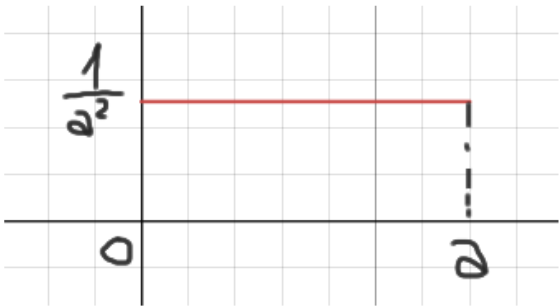
\includegraphics[scale=0.6]{03-TransformadaDeLaplace/3a1.png}
    
    Mirando esto, podemos sacar partido de la función escalón unitario, y redefinir a la función en términos de ella:
    
    $\displaystyle y(t)=\frac{1}{a^{2}}E(t)-\frac{1}{a^{2}}E(t-a)$
    
    Básicamente, lo que estamos haciendo es multiplicar a nuestra función por una función escalón unitario, lo cual nos daría todo el trozo que corresponde a su dominio, y luego, le restamos la parte que no consideramos (ya que para valores mayores a $a$, la función es 0).
    
    Algo a considerar es que no hace falta ``restar'' la parte de $t<0$, ya que la función escalón unitario está definida para $t \geq 0$.
    
    Luego, transformamos la función que tenemos. 
    
    \textbf{\underline{NOTA:}} 
    
    $\displaystyle \lapl{E(t)}=\frac{1}{s}$
    
    $\displaystyle \lapl{E(t-a)}=\frac{e^{-as}}{s}$
    
    $\displaystyle \lapl{y(t)}=\frac{1}{a^{2}} \cdot \frac{1}{s}+ \frac{1}{a^{2}} \cdot \frac{e^{-as}}{s} \implies$
    \fcolorbox{black}{yellow}{$\displaystyle Y(s)=\frac{1-e^{-as}}{a^{2}s}$}
    
    \subsubsection{3b}
    $y(t)=\sen \left(5t+\frac{\pi}{3} \right)\;;\;t>0$
    
    Para resolver este ejercicio, hay que darse cuenta que no se puede aplicar la segunda propiedad de la traslación, ya que no se cumplen las condiciones para poder aplicarla.
    
    Resulta, entonces, que hay que hacer un paso extra para poder transformar esta función. En este caso, basta con aplicar el seno de la suma:
    
    $\displaystyle y(t)=\sen \left(5t\right)\cdot \cos\left(\frac{\pi}{3}\right)+ \sen\left(\frac{\pi}{3}\right)\cdot\cos\left(5t\right)$
    
    Calculamos los números: $\displaystyle y(t)=\frac{1}{2}\sen(5t)+\frac{\sqrt{3}}{2}cos(5t)$
    
    Transformamos usando la tabla: $\displaystyle Y(s)=\frac{1}{2}\frac{5}{s^{2}+25}+\frac{\sqrt{3}}{2}\frac{s}{s^{2}+25}\implies$ \fcolorbox{black}{yellow}{$\displaystyle Y(s)=\frac{\sqrt{3}s+5}{2\left(s^{2}+25\right)}$}
    
    \subsubsection{3c}
    $y(t)=\cos^{3}(t)$
    
    Se puede proceder de muchas maneras para resolver este ejercicio. Yo voy a optar por transformar esta expresión en una equivalente.
    
    Si usamos la forma exponencial del coseno: (recordar) $\displaystyle cos(a)=\frac{e^{aj}+e^{-aj}}{2}$
    
    $\displaystyle y(t)=\left(\frac{e^{jt}+e^{-jt}}{2}\right)^{3}
    =\frac{e^{3jt}}{8}+\frac{3e^{2jt}\cdot e^{-jt}}{8}+\frac{3e^{jt}\cdot e^{-2jt}}{8}+\frac{e^{-3jt}}{8}$
    
    Operando, ordenando y agrupando convenientemente: $\displaystyle y(t)=
    \frac{\highlight{yellow}{ e^{3jt}+e^{-3jt}}}{\highlight{yellow}{2}\cdot4}+\frac{3\left( \highlight{green}{e^{jt}+e^{-jt}} \right)} {\highlight{green}{2}\cdot4}$
    
    Si nos damos cuenta, lo sombreado con amarillo y con verde, representan también la forma exponencial de un coseno, entonces, lo reemplazamos:
    
    $\displaystyle y(t)=\frac{1}{4}\cos(3t)+\frac{3}{4}\cos(t)$
    
    Ahora, estamos en condiciones de transformar directamente: \fcolorbox{black}{yellow}{$\displaystyle Y(s)=\frac{1}{4}\cdot \frac{s}{s^{2}+9}+\frac{3}{4}\cdot \frac{s}{s^{2}+1}$}
    
    \subsubsection{3d}
    $y(t)=a^{t} \; ; \; t>0 \; ; \; a \in \mathbb{R}^{+}$
    
    Aplicamos logaritmo a ambos miembros
    
    $\ln(y(t))=t \ln(a)$
    
    $ \displaystyle e^{\ln(y(t))}=e^{t\cdot ln(a)} \implies y(t)=e^{\ln(a)t}$
    
    ¡Que no panda el cúnico! el $\ln(a)$ es un número! Entonces, podemos transformar directamente usando la tabla para la exponencial:
    
    \fcolorbox{black}{yellow}{$\displaystyle Y(s)=\frac{1}{s-\ln(a)}$}
    
    \subsubsection{3e}
    $y(t)=(t-1)^{4} \; ; \; t>0$
    
    Este ejercicio es una variante del ejercicio 2d. ¿Cuál es la diferencia? El dominio donde está definida la función. Para el ejercicio 2d, decía claramente $t>1$, de forma tal que podíamos aplicar la segunda propiedad de la traslación.
    
    En este caso, no coincide el desplazamiento de la función, con el dominio. Por ende, no se cumplen las hipótesis para aplicar la propiedad.
    
    ¿Qué hacemos? Desarrollamos el binomio y transformamos el resultado. Entonces:
    
    $y(t)=t^{4}-4t^{3}+6t^{2}-4t+1$
    
    $\displaystyle \lapl{y(t)}=\frac{4!}{s^{5}}-4\frac{3!}{s^{4}}+6\frac{2!}{s^{3}}-4\frac{1!}{s^{2}}+\frac{1}{s}$
    
    \fcolorbox{black}{yellow}{$\displaystyle Y(s)=\frac{24}{s^{5}}-\frac{24}{s^{4}}+\frac{12}{s^{3}}-\frac{4}{s^{2}}+\frac{1}{s}$}
	
	\subsubsection{3f}
	$y(t)=\sen(5t)\cos(2t)\;;\;t>0$
	
	Para este último ejercicio no tenemos una transformada directa. Entonces,toca aplicar alguna identidad trigonométrica, ya que tenemos un seno y un coseno.
	
	Tengamos en cuenta: \fcolorbox{black}{white}{$\displaystyle \sen(a)\cdot \cos(b) = \frac{\sen(a-b)+\sen(a+b)}{2}$}
	
	Usamos la identidad:
	$\displaystyle y(t)=\frac{1}{2}\sen(5t-2t)+\frac{1}{2} \sen(5t+2t)$
	
	$\displaystyle y(t)=\frac{1}{2}\sen(3t)+\frac{1}{2} \sen(7t)$
	
	Estas dos funciones ya son transformables:
	
	$\displaystyle Y(s)=\frac{3}{2(s^{2}+9)}+\frac{7}{2(s^{2}+49)}=\frac{3(s^{2}+49)+7(s^{2}+9)}{2(s^{2}+9)(s^{2}+49)}=\frac{3s^2+147+7s^2+63}{2(s^2+9)(s^2+49)}$
	
	Por último: \fcolorbox{black}{yellow}{$\displaystyle Y(s)=\frac{5s^2+105}{(s^2+49)(s^2+9)}$}
	
	\subsection{Ejercicio 4}
	Sea $\displaystyle f(t)=k\sen\left(2t+\frac{\pi}{6}\right)$. Determine el valor de $k$ sabiendo que $\lim\limits_{s \rightarrow \infty} sF(s)=4$.\\
	Recuerde el teorema de valor inicial.
	
	Tal como sugiere el ejercicio, debemos aplicar el teorema de valor inicial. ¿Qué nos decía?
	
	Decía que: $\lim\limits_{t \rightarrow 0} f(t)=\lim\limits_{s \rightarrow \infty}sF(s)$
	
	A nosotros nos están dando como dato el miembro derecho de la igualdad. Entonces queda calcular el límite del miembro izquierdo.
	
	$\displaystyle \lim\limits_{t \rightarrow 0}k\sen\left(2t+\frac{\pi}{6}\right)=4 \implies k\cdot\sen\left(\frac{\pi}{6}\right)=4 \implies k\cdot \frac{1}{2}=4 \implies$
	\fcolorbox{black}{yellow}{$k=8$}
	
	\section{Parte 2: Antitransformada de Laplace - Propiedades}
	\subsection{Ejercicios 5afg}
	Calcule las Antitransformadas de Laplace de las siguientes funciones.
	
	\subsubsection{5a}
	$\displaystyle Y(s)=\frac{25}{s^{3}}$
	
	Para los ejercicios de Antitransformada, siempre hay que mirar la tabla de transformadas, pero ``al revés''. Es muy parecido a como hicimos para las transformadas. A veces puede darse el caso en que necesitemos hacer algún paso algebráico o, como vamos a ver en el ejercicio 6, aplicar fracciones simples.
	
	Para este caso, primero aplicamos linealidad, y luego hacemos la antitransformada directa:
	
	$\displaystyle \ilapl{Y(s)}=25\ilapl{\frac{1}{s^{3}}}$
	
	Por definición, $\ilapl{Y(s)}=y(t)$. Luego, para antitransformar la otra función, necesitamos un $2$ en el numerador. Como no lo tenemos, lo generamos y luego compensamos:
	
	$\displaystyle y(t)=\frac{25}{2}\ilapl{\frac{2}{s^{3}}} \implies$ \fcolorbox{black}{yellow}{$\displaystyle y(t)=\frac{25}{2}t^{2}$}
	
	\subsubsection{5f}
	$\displaystyle Y(s)=\frac{s+3}{s^{2}+6s+13}$
	
	Esta función si la observamos minuciosamente se puede asemejar (aunque no es igual) a un coseno transformado.
	
	En el denominador, podemos llegar a formar un trinomio cuadrado perfecto. Tenemos el $s^{2}$ y el $6s$, el término independiente es incorrecto.
	
	Si no te acordás como formarlo, una ayudita rápida:
	
	Tomamos el coeficiente del término lineal: $6$, y lo dividimos entre $2$: $\frac{6}{2}=3$. A este resultado, lo elevamos al cuadrado $3^{2}=\boxed{9}$
	
	Este último número es el que debemos usar para tener un trinomio cuadrado perfecto. Entonces, para obtenerlo, vamos a separar el término independiente del denominador en $9+4$:
	
	$\displaystyle Y(s)=\frac{s+3}{s^{2}+6s+9+4}=\frac{s+3}{(s+3)^{2}+4}$
	
	Ahora sí, esto se parece mucho más a un coseno, lo que tiene es que está desplazado. ¿Te acordás que propiedad genera un desplazamiento en el dominio de Laplace?
	
	Pensalo 3 segundos...
	3...\\
	2...\\
	1...\\
	
	¡Si! La \textbf{primera propiedad de la traslación}. Ahora, la tenemos que aplicar a la inversa.
	
	\textbf{ATENCIÓN, IMPORTANTE!!!!!:} para poder aplicar la propiedad, en el caso del coseno necesitamos que \textbf{\underline{TODAS}} las $s$ estén desplazadas. Es decir, que si tengo: $\displaystyle Y(s)=\frac{s}{(s+3)^{2}+4}$ no podríamos aplicar la propiedad, en principio. Tendríamos que aplicar una serie de pasos algebraicos adicionales (ya tendremos la oportunidad de hacerlos, en este caso, está hecho a propósito).
	
	Dicho esto, antitransformamos. El tip que va a servirte es que antitransformemos haciendo de cuenta que en vez de $s+3$ tenemos $s$, y luego, en el dominio del tiempo hacemos la corrección que haga falta.
	
	$\displaystyle \ilapl{Y_{2}(s)}=\ilapl{\frac{s}{s^{2}+4}} \implies y_{2}(t)=\cos(2t)$
	
	Para obtener la $y(t)$, multiplicamos por la exponencial de la propiedad: \fcolorbox{black}{yellow}{$y(t)=e^{-3t}\cos(2t)$}
	
	\subsubsection{5g}
	$\displaystyle Y(s)=\frac{s-1}{s^{2}+2s+2}$
	
	Este ejercicio va a servir para poner en ejemplo la advertencia que hicimos en el anterior.
	
	Vamos primero a armar el trinomio cuadrado perfecto del denominador:
	
	$\displaystyle Y(s)=\frac{s-1}{s^{2}+2s+1+1}=\frac{s-1}{(s+1)^{2}+1}$.
	
	En este caso, vemos que no coinciden las ``s'', ya que una es $s+1$ y la otra $s-1$. No podemos aplicar la propiedad (directamente).
	
	Entonces, vamos a hacer una jugarreta. En el numerador sumamos y restamos 1:
	
	$\displaystyle Y(s)=\frac{s-1+1-1}{(s+1)^{2}+1} \;\;\;$. Agrupamos convenientemente: $\displaystyle Y(s)=\frac{s+1-2}{(s+1)^{2}+1}$
	
	Distribuyendo: $\displaystyle Y(s)=\frac{s+1}{(s+1)^2+1}-\frac{2}{(s+1)^2+1}$
	
	Y ahora si, podemos antitransformar directamente, considerando la traslación como hicimos en el ejercicio anterior:
	
	\fcolorbox{black}{yellow}{$y(t)=\cos(t)e^{-t}-2\sen(t)e^{-t}$}
	
	\subsection{Ejercicios 6bij}
	Calcule las Antitransformadas de Laplace de las siguientes funciones previamente separando en fracciones simples.
	
	\subsubsection{6b}
	$\displaystyle Y(s)=\frac{s^{2}+2s+2}{s^{2}+3s+2}$
	\subsubsection{6i}
	$\displaystyle Y(s)=\frac{-2s^{2}+8s-14}{(s+1)(s^{2}-2s+5)}$
	\subsubsection{6j}
	$\displaystyle Y(s)=\frac{(4s+2)e^{-2s}}{(s-1)(s+2)}$
	
	\section{Parte 3: Resolución de ecuaciones diferenciales}
	\section{Parte 4: Convolución}
	\section{Parte 5: Evaluación de integrales}
	\section{Ejercicios bonus}
	\section{Ejercicios para curiosos}
\end{document}
